\section{Les données à notre disposition}

Les données du problème concernent les contentrations de trois types de polluants ($NO_2$, $PM_{10}$, $PM_{2,5}$) sur une période de temps T donnée dans six villes inconnues, numérotées de 0 à 5.
Chaque ville comporte 4 ou 5 stations (29 au total sur les six villes, numérotées de 1 à 29).

\subsection{Variables explicatives}

Pour chacune des stations, nous avons les variables explicatives suivantes:
\begin{itemize}
  \item 19 variables statiques, qui nous renseignent sur l'entourage du point où les mesures sont faites:
  \begin{itemize}
    \item la surface cumulée de zones résidentielles à faible densité dans un rayon de 25/50/150/250/500 mètres autour du point
    \item la surface cumulée de zones résidentielles à haute densité dans un rayon de 25/50/150/250/500 mètres autour du point
    \item la surface cumulée de zones industrielles dans un rayon de 500 mètres autour du point
    \item la surface cumulée de zones portuaires dans un rayon de 2500 mètres autour du point
    \item la surface cumulée d'espaces verts dans un rayon de 2500 mètres autour du point
    \item la distance cumulée de routes dans un rayon de 50/150/250/500 mètres autour du point
    \item l'inverse de la distance à la route la plus proche
  \end{itemize}
  \item 9 variables dynamiques, dont on a les valeurs sur pratiquement toute la periode T, à intervalles de temps d'une heure:
  \begin{itemize}
    \item La température
    \item La vitesse du vent
    \item l'orientation du vent, via la valeur du cosinus et du sinus de l'angle par rapport à une référence inconnue
    \item l'ennuagement
    \item l'intensité des précipitations
    \item la probabilité de précipitations
    \item la pression
    \item une variable booléenne qui indique si le jour est calme ou non
  \end{itemize}
\end{itemize}

\subsection{Données d'entrainement}

Comme données d'entrainement, nous avons les concentrations en polluants à intervalle de temps d'une heure sur toute la période pour 2 ou 3 stations par ville (17 sur 29 au total) pendant 1 an et demi environ.
Pour les 12 autre stations (2 par ville), nous n'avons \textbf{aucune} valeur de concentration en polluants, que nous devons prédire sur les \textbf{mêmes} temps, avec par conséquent les mêmes données dynamiques. En effet, à une heure donnée, les données météorologique (température, vent, pression, ennuagement) sont rigoureusmenent les mêmes pour toutes les stations d'une zone. Ce sont donc uniquement les données statiques qui différencient les stations les unes des autres, y compris pour les stations d'entrainement et de test. %A verifier

\subsection{Problème posé}

Le problème est un problème de régression très général : étant données les variables explicatives et l'évolution temporelle des concentrations en polluants à certain points sur une période T, prédire l'évolution temporelle des concentration en d'autre points à partir des données météorologiques et statiques.
Pour ce faire, nous n'avons que très peu d'exemples (2 ou 3 par ville), bien que la période T soit longue.
La tâche s'annonce donc compliquée.

\subsection{Remarques sur les données}

\begin{itemize}
  \item
    Le comportement physiques des trois polluants est très différent.
    Les particules $PM_{2,5}$ et $PM_{10}$ ont une taille entre 1 et 10 micromètres, et sont suffisamment légères pour rester en suspension dans l'atmosphère. Elle sont solubles dans l'eau; la pluie a donc une très grande influence sur leur concentration dans l'air.
    
    Le $NO_2$ est une molécule de taille moléculaire, soit quelques angströms, beaucoup plus petite que les particules, avec une inertie beaucoup plus faible. Elle est de plus bien moins sensible à la pluie que les micro particules.
    
    Le comportement des différents polluants est donc radicalement différent.
    Cela suggère de traiter différemment les microparticules et le $NO_2$.
  \item
    Nous n'avons aucune donnée géographique qui nous renseigne sur la position relative des différents points les uns par rapport aux autre, ni sur la position relative des éléments (par exemples les routes) qui sont dans l'entourage du point auquel est fait la mesure.
   Nous ne pouvons donc pas espérer apprendre les paramètres d'un modèles pertinent utilisant des théories physiques comme la conduction, qui nous permettraient d'avoir des résultats extrêmement précis ; il s'agit d'un pur problème de machine-learning.
	\item
    	Prenons une carte de répartition annuelle du $NO_2$ sur Paris (source : %mettre ref http://www.airqualitynow.eu):
    \begin{center}
    	%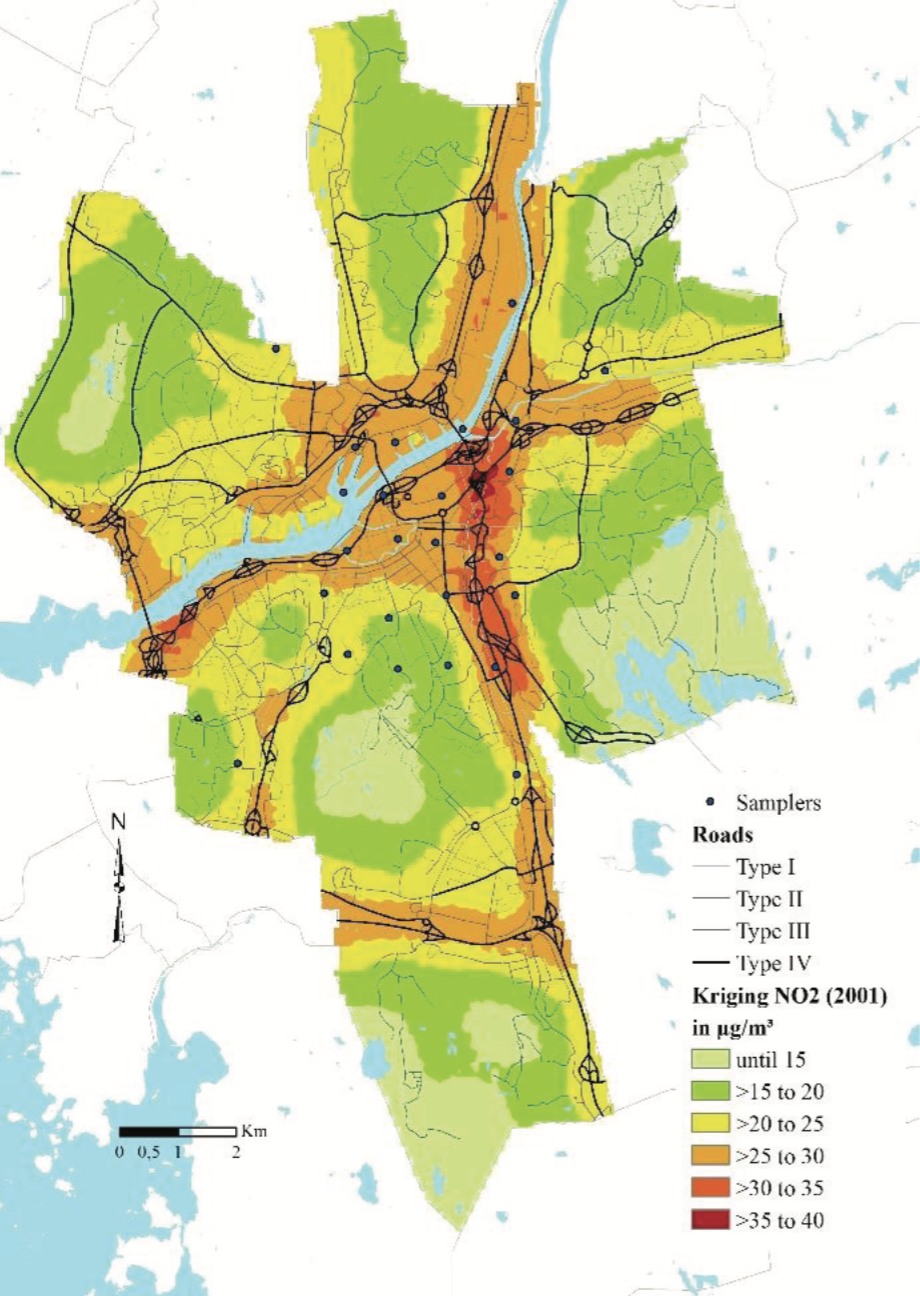
\includegraphics[height=8cm]{images/pollution_gothenburg.png}
    	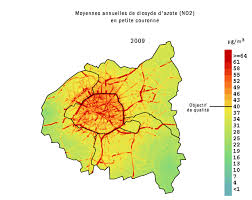
\includegraphics[height=8cm]{images/parisno2.jpg}
    \end{center}
    On constate que la pollution est phénomène spatial, et que le $NO_2$ est principalement concentré autour des grands axes routiers. Il est aussi pertinent de différencier les routes en différentes catégories selon leur fréquentation. Notons au passage que les routes sont classés selon différents types qui semblent être déterminants pour la pollution en $NO_2$, or nous n'avons qu'un type de route à notre disposition, et aucune information sur l'affluence. On peut donc sans aucun doute trouver des points qui auront les même valeurs statiques (surfaces cumulées) et pour lesquels le niveau de pollution est pourtant très différent.    
  \item
    Nous avons fait un script pour vérifier autant que possible la cohérence des données, pour avoir une une idée du niveau de fiabilité des différents paramètres du problème. Nous avons alors repéré que l'angle d'orientation du vent nous est donnée par son cosinus et son sinus, dont la somme des carrés ne font pas 1 en général (moyenne = 0.995, écart type =  0.06 , maximum =  1.995 , minimum = 2.4 $\cdot 10^{-11}$)
 
    
\end{itemize}



\subsection{Exploration des valeurs}

\subsubsection{Influence des données constatées en première approche}
%Faire analyse de l'influence a posteriori, pca, ect...
%Pluie, vent ect..

\subsubsection{Les données dynamiques}

Pour se rendre compte de la répartition des valeurs des données dynamiques, on affiche les histogramme de ces valeurs sur une echelle logarithmique:

% 2 fois pression !
\begin{figure}[H]
	\captionsetup{labelformat=empty}
	\minipage{0.50\textwidth}
	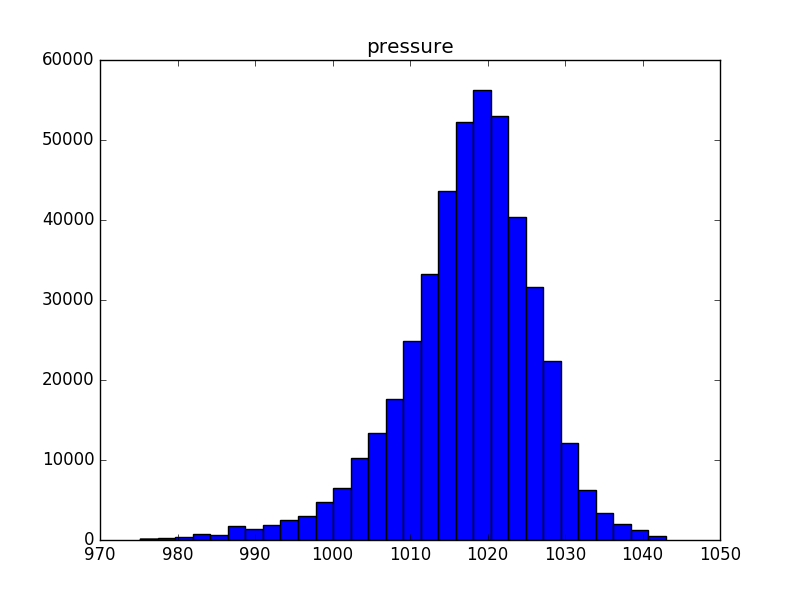
\includegraphics[width=\linewidth]{images/pression.png}
	\caption{pression}
	\endminipage\hfill
	\minipage{0.50\textwidth}
	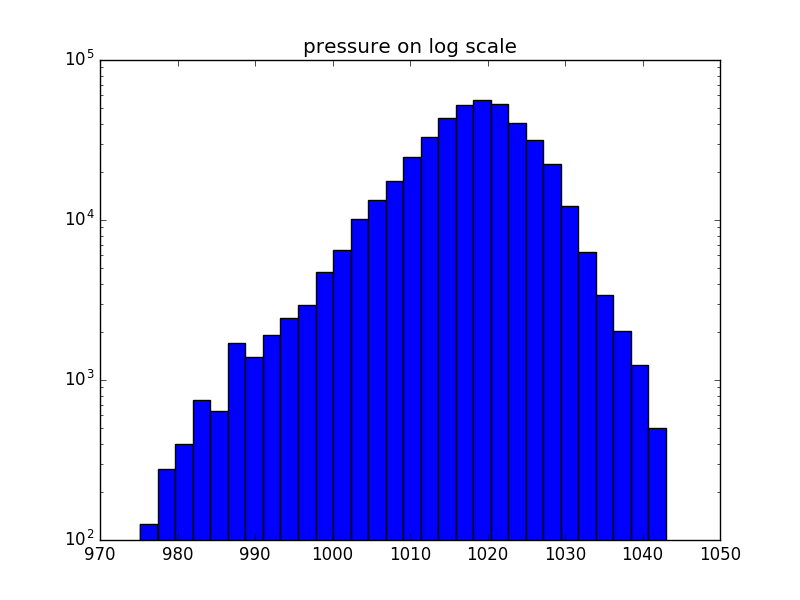
\includegraphics[width=\linewidth]{images/log_pression.png}
	\caption{pression sur échelle log}
	\endminipage\hfill
\end{figure}

\begin{figure}[H]
	\captionsetup{labelformat=empty}
	\minipage{0.50\textwidth}
	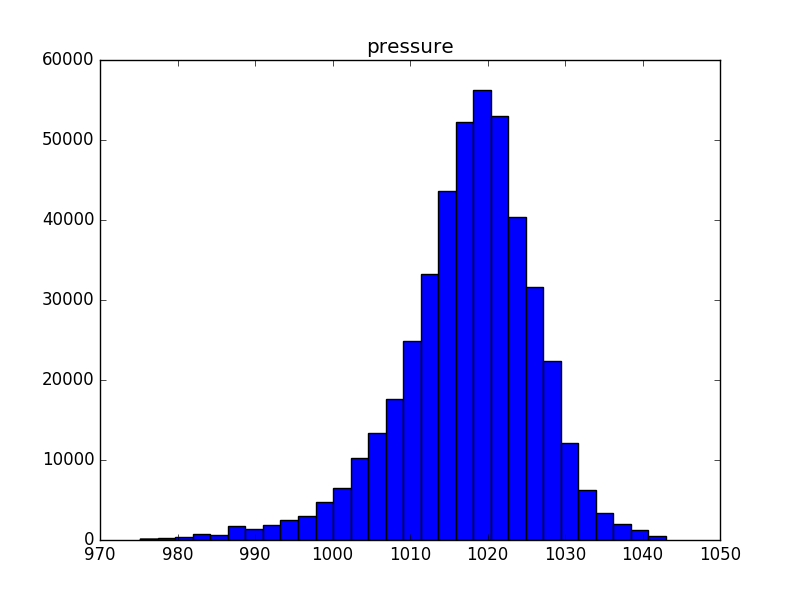
\includegraphics[width=\linewidth]{images/pression.png}
	\caption{pression}
	\endminipage\hfill
	\minipage{0.50\textwidth}
	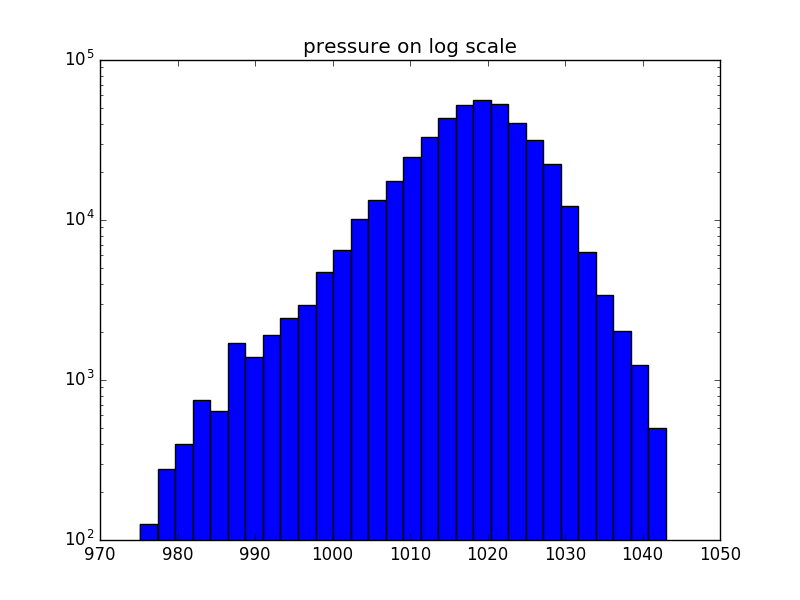
\includegraphics[width=\linewidth]{images/log_pression.png}
	\caption{pression sur échelle log}
	\endminipage\hfill
\end{figure}

\begin{figure}[H]
	\captionsetup{labelformat=empty}
	\minipage{0.50\textwidth}
	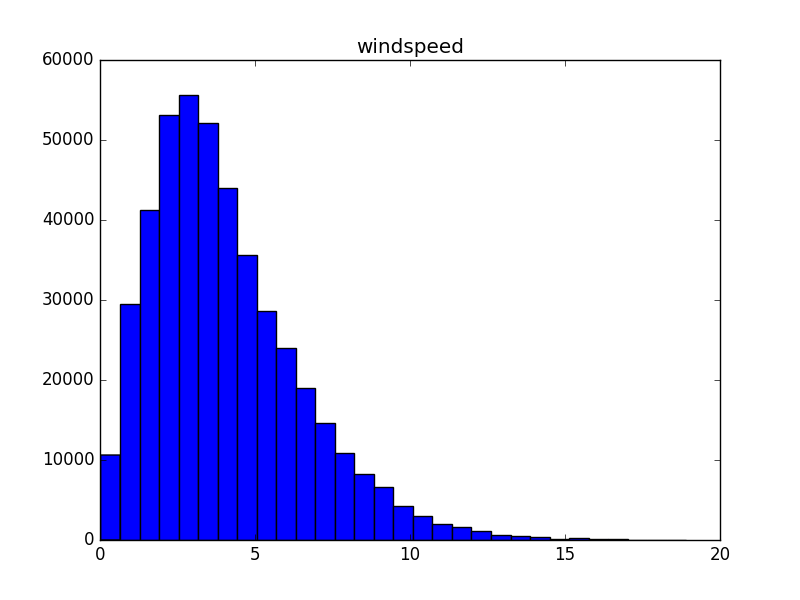
\includegraphics[width=\linewidth]{images/vent.png}
	\caption{vent}
	\endminipage\hfill
	\minipage{0.50\textwidth}
	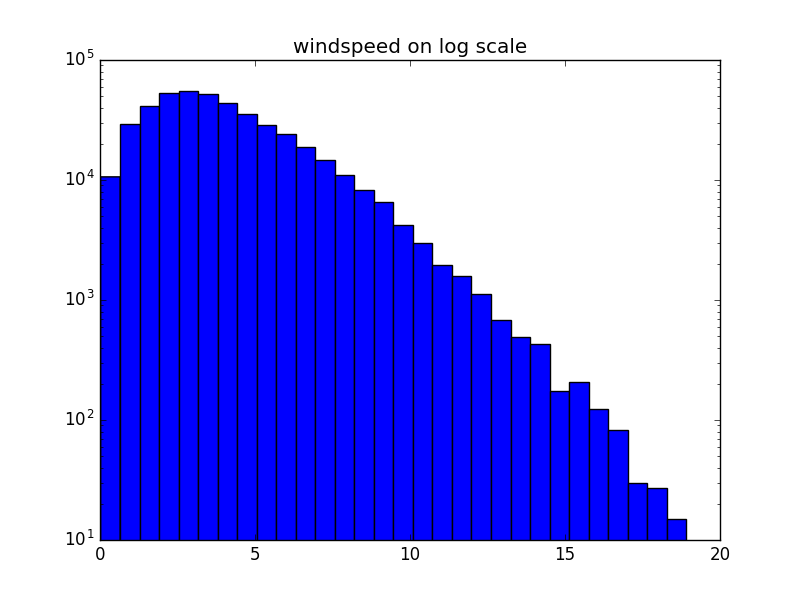
\includegraphics[width=\linewidth]{images/log_vent.png}
	\caption{vent sur échelle log}
	\endminipage\hfill
\end{figure}

\begin{figure}[H]
	\captionsetup{labelformat=empty}
	\minipage{0.50\textwidth}
	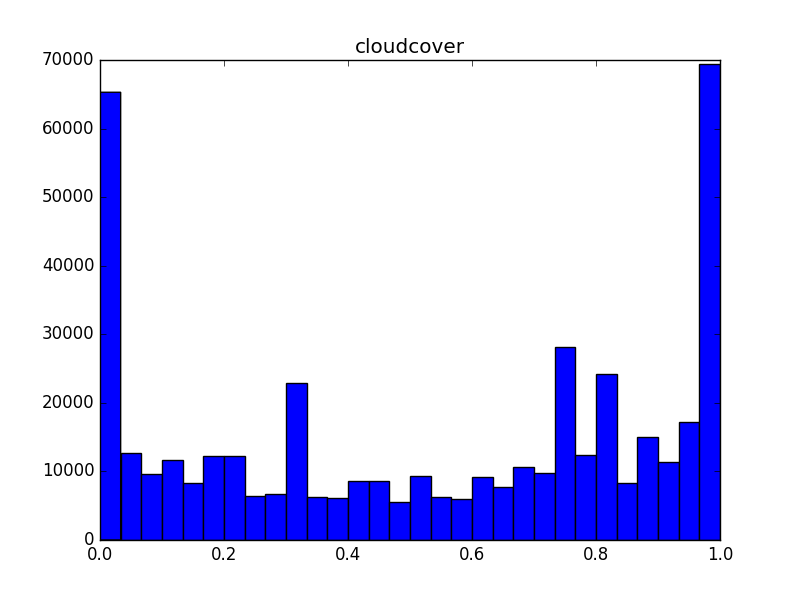
\includegraphics[width=\linewidth]{images/ennuagement.png}
	\caption{ennuagement}
	\endminipage\hfill
	\minipage{0.50\textwidth}
	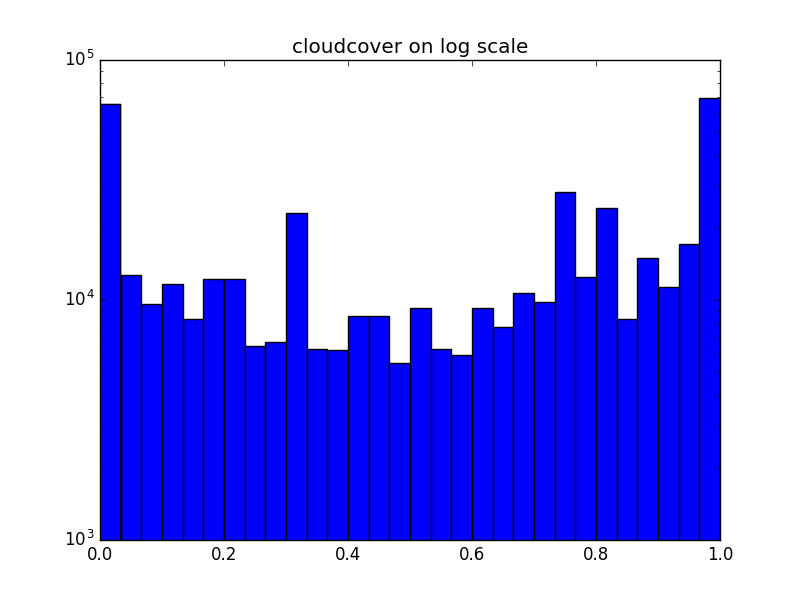
\includegraphics[width=\linewidth]{images/log_ennuagement.png}
	\caption{ennuagement sur échelle log}
	\endminipage\hfill
\end{figure}

\begin{figure}[H]
	\captionsetup{labelformat=empty}
	\minipage{0.50\textwidth}
	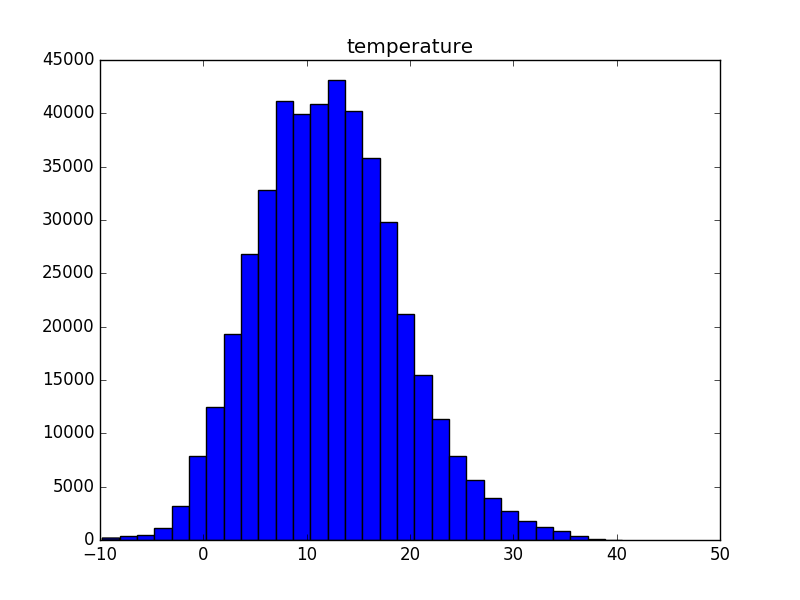
\includegraphics[width=\linewidth]{images/temperature.png}
	\caption{temperature}
	\endminipage\hfill
	\minipage{0.50\textwidth}
	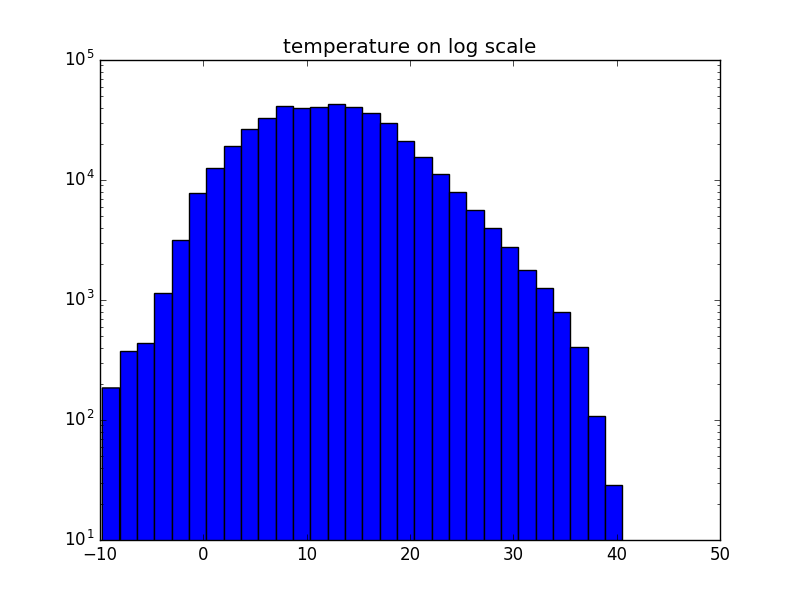
\includegraphics[width=\linewidth]{images/log_temperature.png}
	\caption{temperature sur échelle log}
	\endminipage\hfill
\end{figure}

Il apparaît donc que les données sont plus étalées sur un échelles logarithmique.
Dans la mesure ou nous cherchons à appliques des techniques de régression simples %pourquoi ? expliquer !
et avec une forte régularité (regression lineaire), le fait d'utiliser des échelles logarithmiques est une première transformation que nous pouvons appliquer à nos données avant d'utiliser des modèles de régression simples.

\subsubsection{Les données statiques}

Les données statiques ne sont pas toutes renseignées sur certaines stations. Cela peut être problématique si l'on souhaite utiliser un algorithme d'apprentissage commun à toute les stations. Cependant, nous avons au moins une valeur par catégorie dans les données de type concentration cumulées, ce qui nous a permis d'interpoler les valeurs manquantes. Pour les autres (industrie, port, zones naturelles), les données sont considérées comme nulles si non renseignées, ce qui semble être raisonnable.


\subsection{Conclusion}

En conclusion, les données du problèmes sont peu fiables et discutables. Le fait que les données sur les routes ne soient pas différenciées sera surement un problème pour prédire les concentrations de $NO_2$. De même, partager les même données dynamiques pour toutes les stations d'une zone est discutable, surtout concernant la force et l'orientation du vent, jouant pourtant un rôle essentiel dans l'évolution de la concentration.

Un autre aspect important est cette distinction entre les données statiques (très variées et dont nous disposons que de 29 exemples) et les données dynamiques en grand nombre, identiques par zone, mais non redondantes entre les zones. Cela nous empêche donc d'apprendre un modèle par zone, et nuit à l'apprentissage d'un modèle commun aux zones. Cet aspect est la principale difficulté du problème.  

Nous pouvant ainsi dès à présent anticiper que les prévisions de ce problème resteront très grossières, surtout concernant le $NO_2$.

